\documentclass[10pt,a4paper]{memoir}

\usepackage[left=2.5cm,right=2.5cm,top=2.5cm,bottom=3cm]{geometry}
\usepackage[utf8]{inputenc}
\usepackage{palatino}
\usepackage[T1]{fontenc}
\usepackage{graphicx}
\graphicspath{{../images/}}
\usepackage{hyperref}
\usepackage{amsmath}
\usepackage{amsfonts}
\usepackage{amssymb}


\begin{document}
\setlength{\parindent}{0pt}


% Title page
 \vspace*{3cm}
	
 \begin{center}
 	\HUGE eistoolbox \par
 \end{center}
 \begin{center}
 	\LARGE for \par
 \end{center}
 \begin{center}
 	\HUGE Mathworks\textsuperscript{\textregistered} MATLAB \par
 \end{center}
 
 \vspace*{2cm}
 
\begin{center}
	\Large A toolbox for batch fitting of Electrochemical Impedance Spectroscopy data to equivalent circuit models
\end{center} 
 
 \vspace*{2cm}
 
 \begin{center}
 	\Huge User Guide \par
 \end{center}
 \begin{center}
 	\LARGE Juan J. Montero-Rodríguez \par
 \end{center}
 
 \vspace*{4cm}
 
 \begin{center}
 	\Large Version 0.1-45
 \end{center}

\clearpage




\tableofcontents

\chapter{Introduction}

Electrochemical Impedance Spectroscopy (EIS) is a laboratory technique consisting of acquiring the frequency response of

\textbf{eistoolbox} is a toolbox for MATLAB\textregistered{} used for batch fitting Electrochemical Impedance Spectroscopy (EIS) data to equivalent circuits. 

Presently it is \textbf{alpha software}, and it will evolve over time.

\section{Current capabilities}

It can accept any number of input files, both in CSV and Gamry DTA formats.

The CSV files should contain three columns with the impedance data, in the order: FREQ,REAL,IMAG. 

The imaginary part can be positive or negative; the absolute value is taken inside the program before plotting.

The fitting algorithm uses the "fminsearch" function, implemented using the Zfit library from Jean-Luc Dellis. 

It accepts any type of circuit model, built with serial and parallel elements, in the Zfit circuit string format.

The currently implemented elements are: resistors, capacitors, inductors and constant-phase elements (CPE). 

The Warburg element can be implemented by using a CPE and setting the second parameter to 1/2.


\section{Planned updates}

In the future it will accept Levenberg-Marquard, Nelder-Mead, BFGS and Powell algorithms.

It will also include the error percentages of every fitting parameter, as well as the Pearson coefficient and correlation plot of the fitting results.


\chapter{Using the eistoolbox}

\section{Quick start guide}

1. Add files using the "Add file..." button

2. Write the circuit string and fitting parameters (circuit string formatting)

3. Click the "Fit" button

4. Save the results using the "Save..." button

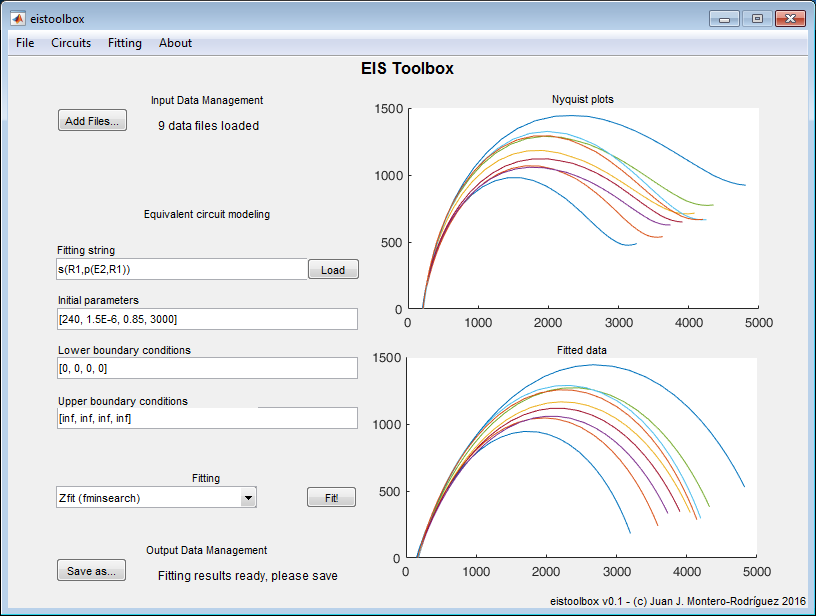
\includegraphics[width=15cm]{main_screenshot.png}

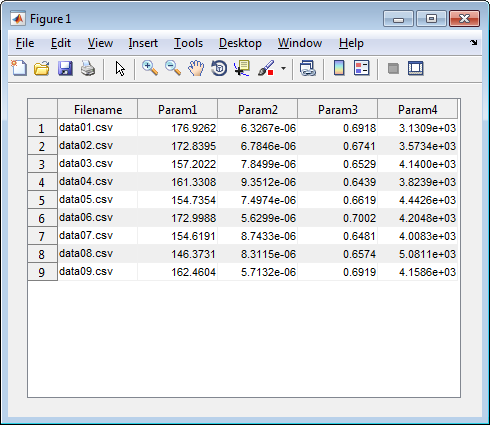
\includegraphics[width=10cm]{scr_results.png}


\chapter{Algorithms}

\section{fminsearchbnd}

Currently it supports only the fminsearchbnd function from Zfit.m


\chapter{Statistics}

The program computes the following statistical parameters:

\section{Linear regressions}

Real of fitted vs Real of measured

Imag of fitted vs Imag of measured

MAG of fitted vs MAG of measured

\section{Chi-square goodness of fit}

\[ \chi^2 = \sum_i^n{\dfrac{(Observed_i-Expected_i)^2}{Expected_i}} \]

Observed= fitted data

Expected= measured data

\section{Error estimates for individual parameters}

ToDo


\newpage{}
\chapter{Licenses for included software}

\section{Zfit}

The original file was released in 2005 and it is available here:\\

\url{https://de.mathworks.com/matlabcentral/fileexchange/19460-zfit}

\begin{small}
\begin{verbatim}
Copyright (c) 2005, Jean-Luc Dellis
All rights reserved.

Redistribution and use in source and binary forms, with or without
modification, are permitted provided that the following conditions are
met:

* Redistributions of source code must retain the above copyright
notice, this list of conditions and the following disclaimer.
* Redistributions in binary form must reproduce the above copyright
notice, this list of conditions and the following disclaimer in
the documentation and/or other materials provided with the distribution

THIS SOFTWARE IS PROVIDED BY THE COPYRIGHT HOLDERS AND CONTRIBUTORS "AS IS"
AND ANY EXPRESS OR IMPLIED WARRANTIES, INCLUDING, BUT NOT LIMITED TO, THE
IMPLIED WARRANTIES OF MERCHANTABILITY AND FITNESS FOR A PARTICULAR PURPOSE
ARE DISCLAIMED. IN NO EVENT SHALL THE COPYRIGHT OWNER OR CONTRIBUTORS BE
LIABLE FOR ANY DIRECT, INDIRECT, INCIDENTAL, SPECIAL, EXEMPLARY, OR
CONSEQUENTIAL DAMAGES (INCLUDING, BUT NOT LIMITED TO, PROCUREMENT OF
SUBSTITUTE GOODS OR SERVICES; LOSS OF USE, DATA, OR PROFITS; OR BUSINESS
INTERRUPTION) HOWEVER CAUSED AND ON ANY THEORY OF LIABILITY, WHETHER IN
CONTRACT, STRICT LIABILITY, OR TORT (INCLUDING NEGLIGENCE OR OTHERWISE)
ARISING IN ANY WAY OUT OF THE USE OF THIS SOFTWARE, EVEN IF ADVISED OF THE
POSSIBILITY OF SUCH DAMAGE.
\end{verbatim}
\end{small}


\end{document}
